% Options for packages loaded elsewhere
\PassOptionsToPackage{unicode}{hyperref}
\PassOptionsToPackage{hyphens}{url}
%
\documentclass[
  a4paper,
  11pt,
  twocolumn]{article}
\usepackage{amsmath,amssymb}
\usepackage{iftex}
\ifPDFTeX
  \usepackage[T1]{fontenc}
  \usepackage[utf8]{inputenc}
  \usepackage{textcomp} % provide euro and other symbols
\else % if luatex or xetex
  \usepackage{unicode-math} % this also loads fontspec
  \defaultfontfeatures{Scale=MatchLowercase}
  \defaultfontfeatures[\rmfamily]{Ligatures=TeX,Scale=1}
\fi
\usepackage{lmodern}
\ifPDFTeX\else
  % xetex/luatex font selection
\fi
% Use upquote if available, for straight quotes in verbatim environments
\IfFileExists{upquote.sty}{\usepackage{upquote}}{}
\IfFileExists{microtype.sty}{% use microtype if available
  \usepackage[]{microtype}
  \UseMicrotypeSet[protrusion]{basicmath} % disable protrusion for tt fonts
}{}
\makeatletter
\@ifundefined{KOMAClassName}{% if non-KOMA class
  \IfFileExists{parskip.sty}{%
    \usepackage{parskip}
  }{% else
    \setlength{\parindent}{0pt}
    \setlength{\parskip}{6pt plus 2pt minus 1pt}}
}{% if KOMA class
  \KOMAoptions{parskip=half}}
\makeatother
\usepackage{xcolor}
\usepackage{graphicx}
\makeatletter
\def\maxwidth{\ifdim\Gin@nat@width>\linewidth\linewidth\else\Gin@nat@width\fi}
\def\maxheight{\ifdim\Gin@nat@height>\textheight\textheight\else\Gin@nat@height\fi}
\makeatother
% Scale images if necessary, so that they will not overflow the page
% margins by default, and it is still possible to overwrite the defaults
% using explicit options in \includegraphics[width, height, ...]{}
\setkeys{Gin}{width=\maxwidth,height=\maxheight,keepaspectratio}
% Set default figure placement to htbp
\makeatletter
\def\fps@figure{htbp}
\makeatother
\setlength{\emergencystretch}{3em} % prevent overfull lines
\providecommand{\tightlist}{%
  \setlength{\itemsep}{0pt}\setlength{\parskip}{0pt}}
\setcounter{secnumdepth}{5}
%------------------------------------------------------------------------------%
% PAPER TEMPLATE FOR ICPHS 2023 Prague                                         %
%                                                                              %
% Original template downloaded from:                                           %
% http://www.icphs2023.org/call-for-papers/                                    %
%                                                                              %
% Reformatted to work with Rmarkdown and R by:                                 %
% Joseph V. Casillas | Rutgers Univesity |11/11/2022                           %
%                                                                              %
% Available for download at:                                                   %
% https://github.com/jvcasillas/icphs2023_rmd_template                         %
%------------------------------------------------------------------------------%



% Packages
\usepackage{./includes/tex/icphs2023}
\usepackage{metalogo} 
\usepackage{epstopdf}
\usepackage{tipa}

% Links and urls must be black
%\hypersetup{urlcolor=black, citecolor=black, linkcolor=black}


% Packages removed from icphs2023.sty because of conflicts
% They have been added to the .Rmd yaml front matter
% \usepackage[latin1]{inputenc}
% \usepackage[T1]{fontenc}
% \usepackage[leqno,fleqn]{amsmath}
\usepackage[utf8]{inputenc}
\usepackage[T1]{fontenc}
\ifLuaTeX
  \usepackage{selnolig}  % disable illegal ligatures
\fi
\usepackage{bookmark}
\IfFileExists{xurl.sty}{\usepackage{xurl}}{} % add URL line breaks if available
\urlstyle{same}
\hypersetup{
  hidelinks,
  pdfcreator={LaTeX via pandoc}}

\author{}
\date{\vspace{-2.5em}}

\begin{document}

\title{Exploring AI-generated voice stimuli and their potential use in the SLA field: Can L2 learners discriminate between AI and human-generated voice?}
\author{Jorge L. Vargas-Mutizabal}
\organization{Rutgers University}
\email{jorge.vargas@rutgers.edu}


\maketitle

\begin{abstract}
This pilot study tested whether undergraduate Spanish learners could determine whether stimuli were produced by AI or a human. The results showed that both groups distinguished between AI and human voice. Additionally, F0 and speech rate were inspected using Praat, and the analysis showed they exhibited similar values. 



\end{abstract}

\keywords{Artificial intelligence (AI), perception, L2 acquisition, phonology (maximally two 
lines).}


\section{Introduction}

Artificial intelligence (AI) is revolutionizing the world, and it is a
developing tool in diverse areas, to name a few: customer service
\cite{wang2023voice}, medical assistance
\cite{longoni2019resistance}(Longoni et al., (2019), and education
\cite{pokrivcakova2019preparing} (Pokrivcakova, 2019), among others. AI
is a subfield of computer science that uses technology to create systems
that emulate human behavior or capacities such as reasoning,
problem-solving, knowledge of languages,
etc.\cite{chowdhary2020fundamentals} (Chowdhary, 2020). The ability of
artificial intelligence to produce language has led to its use in second
language acquisition (L2) as a tool for practice
\cite{fitria2021use}(Fitria, 2021). For example, some studies have
explored its uses to help ESL with their speaking skills
\cite{duong2024effects}(Duong \& Suppasetseree, 2024;
\cite{ccakmak2022chatbot}Çakmak, 2022; \cite{han2020effects}Han, 2020),
showing positive outcomes. However, AI is still a new resource, and
little is known about L2 learners' perception of the AI-generated voices
nor to what extent they share similar phonological features. Therefore,
this pilot study aims to be the first approach to answer whether L2
learners can discriminate between AI and human-generated voices and
whether the voices share the same phonological features. Specifically,
speech rate and F0 values will be explored.

\section{Background}

Human beings interact with AI voice systems both in spoken and written
language. The capacity of AI to generate language has been applied to L2
learning digital platforms where learners can practice their target
languages and improve their proficiency, e.g.~Duolingo, Chatbots, and
Elsa, among others \cite{fitria2021use}(Fitria, 2021). Literature
reporting the outcomes of AI-based L2 language learning is scarce as the
uses of artificial intelligence are still a newly developed resource.
The studies available up to date have focused on English as a second
language (ESL). For instance, the study by \cite{han2020effects} Han
(2020) showed positive results using chatbots to help middle school
students improve their speaking skills in Korea. In particular, the
experiment used Alexa ---the Amazon voice assistant --- to maintain
conversation sessions with the students. Similarly,
(\cite{duong2024effects} Duong \& Suppasetseree (2024) showed that
chatbots helped undergraduate English learners improve their oral
abilities with Andy English bot ---an interactive platform specifically
designed for English learning--- in Vietnam. These two studies
illustrate that AI can have promising applications in the language
classroom, opening a new setting where learners can practice the target
language in a digital environment.

L2 learners' perception of AI is an understudied area, few studies have
explored this matter and are also focused on ESL.
\cite{ccakmak2022chatbot}Çakmak (2022) studied L2 learners' perception
of the Chabot Replika among university students. Their results showed a
negative perception from learners as they had issues being understood by
the platform. However, they had a better performance with the chatbot
than with human interlocutors. A section of \cite{duong2024effects}
Duong \& Suppasetseree (2024) addressed participants' perceptions. They
reported mostly positive impressions emphasizing the availability of AI
for students to practice frequently. Also, learners enjoyed receiving
motivational comments from the chatbot, which helped to keep themselves
engaged with the platform. Among the negative perceptions, the chatbot
had issues repeating their Vietnamese names. From the field of education
but relevant to this study, \cite{kit2023perception} Kit et al., (2023)
explored the perception of higher education students using human voice
and AI voice-generated video for instructional purposes. Their
experiment showed that students preferred the videos with human voice
over AI. Additionally, \cite{zellou2021influence} Zellou et al., (2021)
conducted an experiment framed within phonology alignment, which showed
that humans aligned with other humans and not with an AI interlocutor.

The extant literature showed that AI has potential in SLA. However,
little is known about how learners perceive AI-generated voices and no
studies have been conducted in Spanish as an additional language. This
pilot study exploreed Spanish learners' discrimination between AI and
human-generated voice. To ensure that both voices shared similar
features, two phonological aspects were compared: pitch (F0) and speech
rate. These two measures were addressed as a secondary object of study.

\section{Research questions and hypothesis}

The main research question guiding this study was: Can Spanish L2
learners recognize whether stimuli were generated by AI or human? To
what extent the phonological features of speech rate and F0 are similar
or different? With the results reported by \cite{kit2023perception} Kit
et al.~(2023) and \cite{zellou2021influence} Zellou et al., (2021) as
references, it was hypothesized that learners would recognize whether
stimuli were produced by AI or human voice. Regarding the phonological
features, the AI voice platform had a voice available that matched the
sex and variety of the human voice. Therefore, they are expected to
share similar phonetic characteristics.

\section{Methods}

The stimuli were prepared by randomly selecting 10 tokens from a pool of
384 noun phrases with adjectives (half masculine/half feminine), e.g.~el
barco rápido / la ciudad fría. The 10 phrases were recorded by a female
peninsular Spanish native speaker in a whisper room 6084 E sound booth,
and the same phrases were produced by one of the peninsular Spanish
female voices available on the Natural Readers software. To compare the
speech rate for both voices, the Praat script by \cite{de2009praat} De
Jong \& Wempe (2009) was used, while F0 means were obtained manually by
selecting the phrase sound on Praat and tabulated in a csv file. The
surveys were implemented on Qualtrics where the AI and human-generated
voices were randomly listed (n=20). The sound files only played once,
with the modification of the Qualtrics JavaScript. The participants
played the sound and selected either human or AI voice.

\section{Participants}

The participants for this pilot study were 18 subjects from the Spanish
in the World class (160), which has both L2 learners and heritage
speakers (139) (no requirements to take the class), and 10 subjects from
a heritage speakers' class. No information about their proficiency
levels was available, but the former class is taught in English and the
latter in Spanish.

\section{Results}

The survey had a total of 20 points, and the average mean result for the
participants was 17.5 and 16.8 for the Spanish in the World (160) and
Heritage Speaker (139) classes respectively. These high results indicate
that both groups were able to discriminate between AI and
human-generated voices. The 160 course is given online, therefore they
took the surveys from home, while the Span (139)took the survey in
class.

\begin{figure}[!ht]
\begin{center}
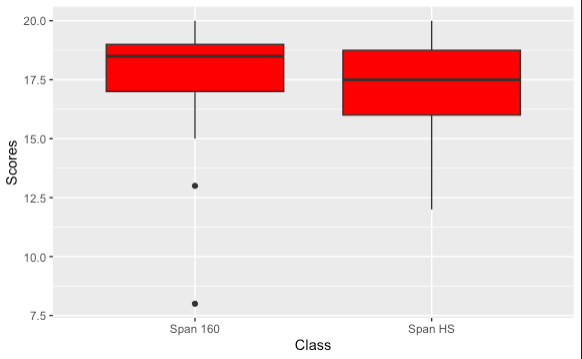
\includegraphics[width=6cm]{./includes/figures/mean.png}
\caption{Figure 1. Survey means values for Span (160) and 139 classes.}\label{fig:vowels}
\end{center}
\end{figure}

A closer look at the incorrect answers showed that 8 out of 18
participants of the Spanish 139 class, had question 2 wrong (n=8), while
there is not much variability of trends with other questions.

\begin{figure}[!ht]
\begin{center}
\includegraphics[width=6cm]{./includes/figures/incorrect plot.png}
\caption{Figure 2. Figure 2. Count of incorrect answers for Span (160) and 139 classes}\label{fig:vowels}
\end{center}
\end{figure}

The phonological features showed similar values for both voices. Speech
rate provides values in syllables per second, resulting in 3.88 for AI
and 3.62 for the human voice.

\begin{figure}[!ht]
\begin{center}
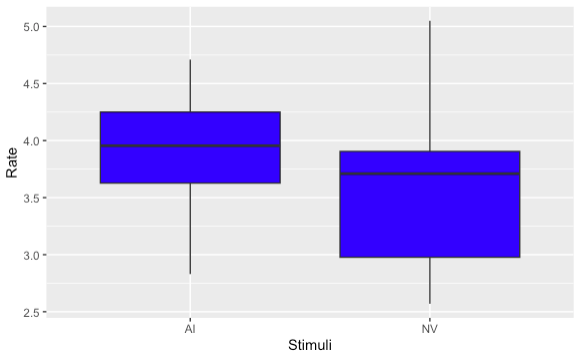
\includegraphics[width=6cm]{./includes/figures/rate.png}
\caption{Figure 3. Speech rate mean values for Span (160) and 139 classes}\label{fig:vowels}
\end{center}
\end{figure}

Pitch (F0) was also found at a similar level, the mean for AI was 199.52
Hz and 204.51 Hz for the human voice.

\begin{figure}[!ht]
\begin{center}
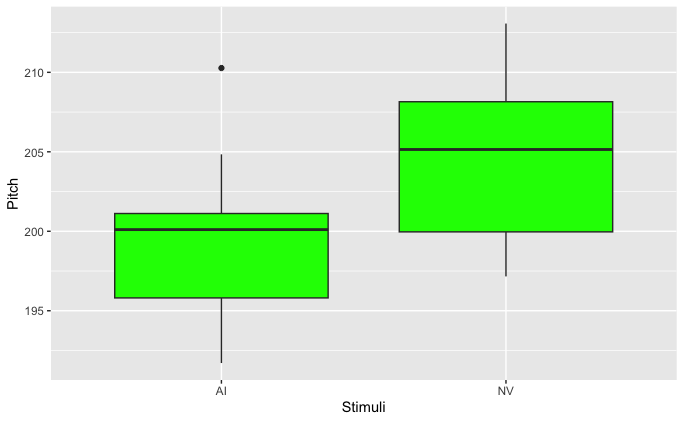
\includegraphics[width=6cm]{./includes/figures/pitch}
\caption{Figure 4. Pitch means values for Span (160) and 139 classes}\label{fig:vowels}
\end{center}
\end{figure}

\section{Discussion}

With AI technology being used more often in most areas of society,
including second language teaching, this pilot study aimed to answer
whether Spanish learners can discriminate between AI voice and human
voice. The mean results for the two Spanish L2 learners' courses were
high: Span 160 with 17.5 and Span 139 with 16.8 out of 20 points. In
agreement with the hypothesis, these results indicate that most learners
in the two classes can accurately discriminate between AI voice and
human voice stimuli. Even though learners might prefer a human voice
\cite{kit2023perception} Kit et al.~(2023), and they might be able to
distinguish when they are listening to an AI voice, studies have shown
that interaction with an AI voice can be useful to improve speaking
skills in the L2 \cite{duong2024effects,}(Duong \& Suppasetseree, 2024;
\cite{han2020effects} Han, 2020). AI produced the first two stimuli from
the experiment, and the third was the human voice. Figure 2, showed that
stimulus number 2 in the survey was incorrectly perceived as a human
voice by 8 learners from Span 160, representing the stimulus with the
most incorrect answers. This trend indicates that some learners might
have tried to guess at the beginning of the survey, and after hearing
the third stimulus with the human voice they might have noticed the
difference in the voices. This means learners might have relied on the
voice contrast to select the correct choice. Interestingly, this trend
only occurred with the Span 160 class and not in the Heritage Speaker
139 class. Due to proficiency scores not being available for these
levels at the moment of data collection or background screening, no
correlations can be made but the nature of the courses provides some
hints. For instance, this opens the question of whether proficiency or
stage of acquisition (late or early bilingual) affects the
discrimination between AI and human voice.

The second objective of this study was to determine to which extent the
AI and human-generated voice are similar or different. In particular,
speech rate and pitch (F0) were explored. In agreement with the
hypothesis, the results showed that both voices had a similar speech
rate, with means values of number of syllables per second of 3.88 for AI
and 3.62. Note that the default settings of 1x were used to produce the
AI sound files. These values show that AI can produce language at a
speech rate similar to a human. The pitch values were also found at a
similar level with 199.52 Hz for AI and 204.51 Hz for the human voice.
However, figure 3 shows that the speech rate range is more variable for
the human voice than for AI. Similarly, figure 4 shows that the pitch of
AI is spread within a smaller range than the human voice. This
observation led to wonder whether the internal structure of each AI has
less variation than human voice which might contribute to a more
monotonous or robotic effect. With the current data, it is not possible
to make further assumptions, but these differences might give the AI
voice a more distinct pitch and a possible hint for learners to
discriminate between the two types of voices.

\section{Conclusion}

The experiment showed that learners from two undergraduate Spanish
courses were able to distinguish between AI and Human-generated voice
stimuli in a survey. However, learners might have relied on contrasting
the two voices to discriminate between AI and Human-generated voices.
Therefore, in the final version of this study, it will be necessary to
create two versions of the experiment: (1) only with AI, (2) only with
human voice, and (3) with both AI and human voice mixed as presented in
this study. This form of experimental design might provide better
insights into whether learners can distinguish the source of a voice.
The speech rate and pitch mean values were similar for AI and human
voice. The mean values showed that despite being comparable, learners
still discriminated between them. However, this experiment did not
consider internal variability within each sound, which in a future study
might provide hints of whether less variability might contribute to
making sounds more monotonous or robotic.

\bibliographystyle{./includes/bib/IEEEtran.bst}
\bibliography{./includes/bib/icphs2023.bib}

\end{document}
